%
%
\pgfplotsset{colormap={cubicyf}{
rgb = (0.5151, 0.0482, 0.66969999999999996)
rgb = (0.52071100000000003, 0.16895499999999999, 0.80057400000000001)
rgb = (0.49369400000000002, 0.27859600000000001, 0.91182399999999997)
rgb = (0.44002599999999997, 0.369475, 0.98497800000000002)
rgb = (0.39893200000000001, 0.45759300000000003, 0.98705299999999996)
rgb = (0.35065099999999999, 0.54064400000000001, 0.92960799999999999)
rgb = (0.29882700000000001, 0.61562499999999998, 0.85772899999999996)
rgb = (0.239928, 0.68506100000000003, 0.76953099999999997)
rgb = (0.22883200000000001, 0.73934900000000003, 0.67328699999999997)
rgb = (0.263297, 0.78608, 0.56998800000000005)
rgb = (0.29810700000000001, 0.82833699999999999, 0.46021400000000001)
rgb = (0.33091999999999999, 0.86407100000000003, 0.35267399999999999)
rgb = (0.38306000000000001, 0.898169, 0.28730899999999998)
rgb = (0.49023, 0.91748099999999999, 0.30796099999999998)
rgb = (0.62372000000000005, 0.92602600000000002, 0.33230900000000002)
rgb = (0.71745800000000004, 0.92527000000000004, 0.342476)
rgb = (0.80000000000000004, 0.92549999999999999, 0.35289999999999999)
}}
\pgfplotsset{colormap={rdoryl}{
rgb(0)=(1, 1, 0.80000000000000004)
rgb(1)=(1, 0.96678200000000003, 0.71879999999999999)
rgb(2)=(1, 0.93134899999999998, 0.63218799999999997)
rgb(3)=(0.998139, 0.89219499999999996, 0.54929600000000001)
rgb(4)=(0.99617100000000003, 0.85282599999999997, 0.46662100000000001)
rgb(5)=(0.99607800000000002, 0.77780899999999997, 0.38394499999999998)
rgb(6)=(0.99607800000000002, 0.70103800000000005, 0.30126900000000001)
rgb(7)=(0.99418700000000004, 0.62805100000000003, 0.26777400000000001)
rgb(8)=(0.99221800000000004, 0.55521699999999996, 0.23627799999999999)
rgb(9)=(0.99024999999999996, 0.43280299999999999, 0.20096900000000001)
rgb(10)=(0.98828099999999997, 0.30878899999999998, 0.16553599999999999)
rgb(11)=(0.94017700000000004, 0.20592099999999999, 0.137793)
rgb(12)=(0.89096500000000001, 0.10356, 0.110235)
rgb(13)=(0.81656300000000004, 0.051580000000000001, 0.12918099999999999)
rgb(14)=(0.741761, 0.00040000000000000002, 0.148866)
rgb(15)=(0.62203799999999998, 0, 0.14902000000000001)
rgb(16)=(0.50196099999999999, 0, 0.14902000000000001)
}}
%
\begin{tikzpicture}
    \tikzstyle{image} = [inner sep=0, outer sep=0, node distance = 0 and 0]

    % place image in node
    \node[image] (image1)
    {
        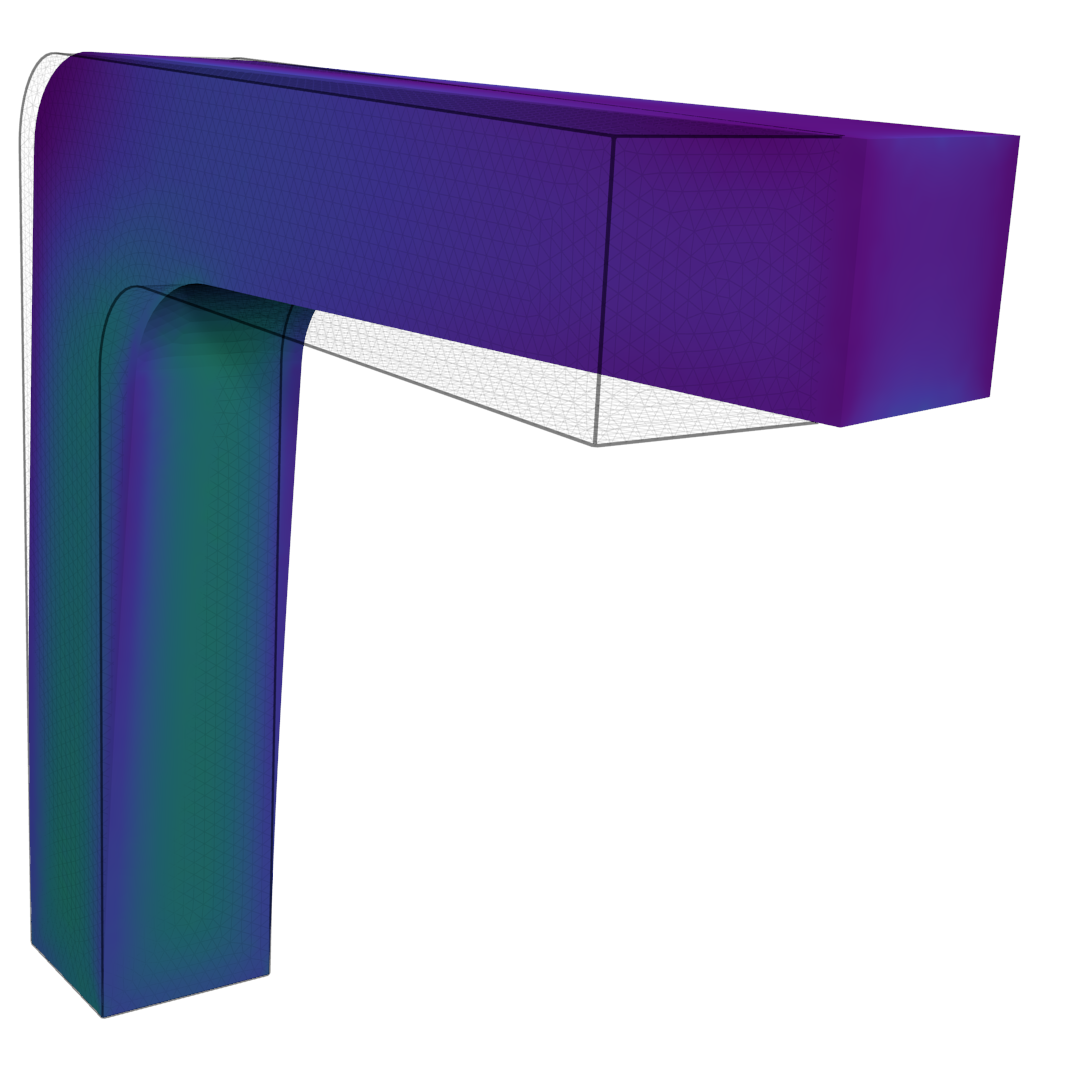
\includegraphics[width=0.22\figurewidth]{figures/hook2_deformation}%
    };

    \node[image, right=of image1, xshift=0.25cm] (image2)
    {
        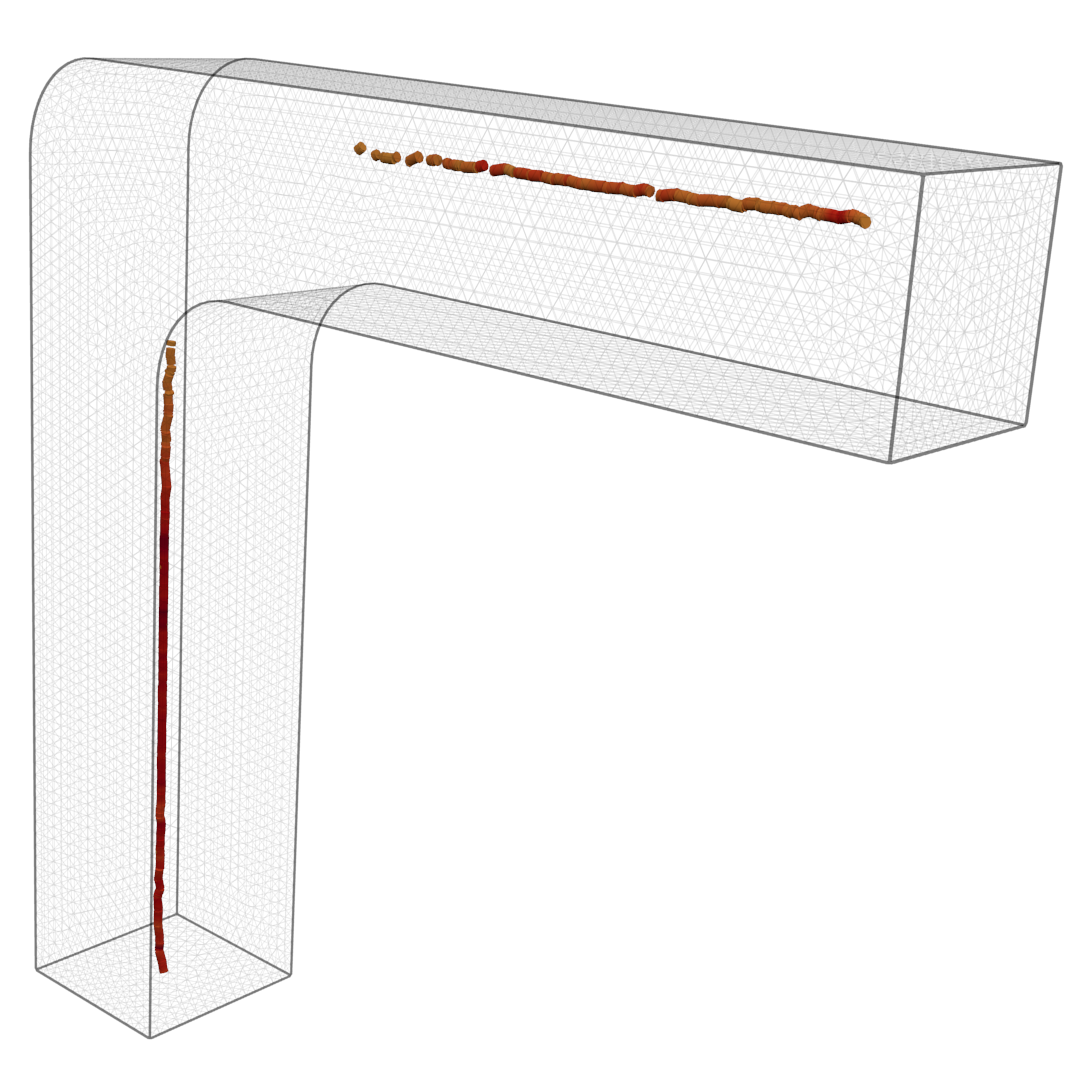
\includegraphics[width=0.22\figurewidth]{figures/hook2_lines}%
    };

    \node[image, right=of image2, xshift=0.25cm] (image3)
    {
        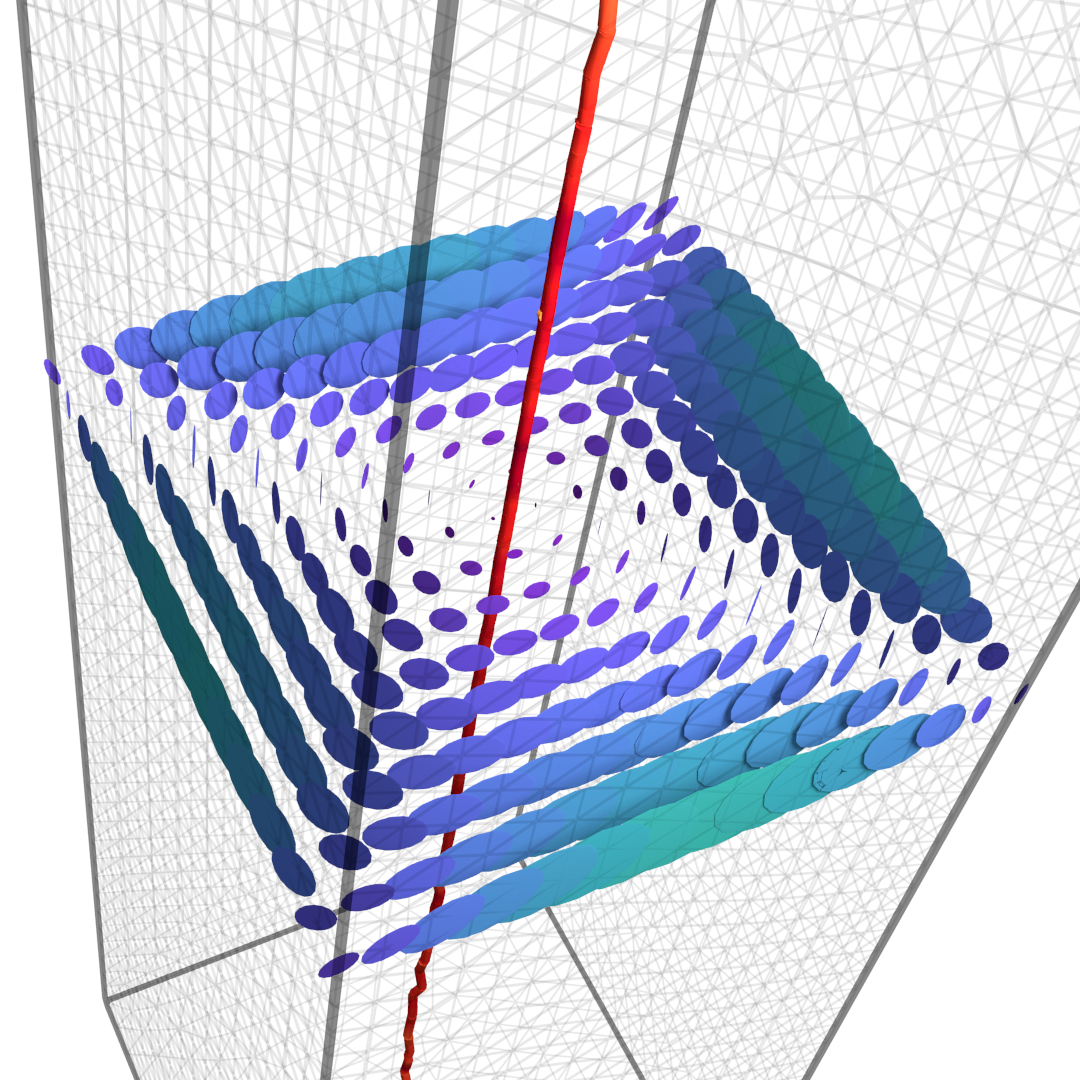
\includegraphics[width=0.22\figurewidth]{figures/hook2_detail1}%
    };

    \node[image, right=of image3, xshift=0.25cm] (image4)
    {
        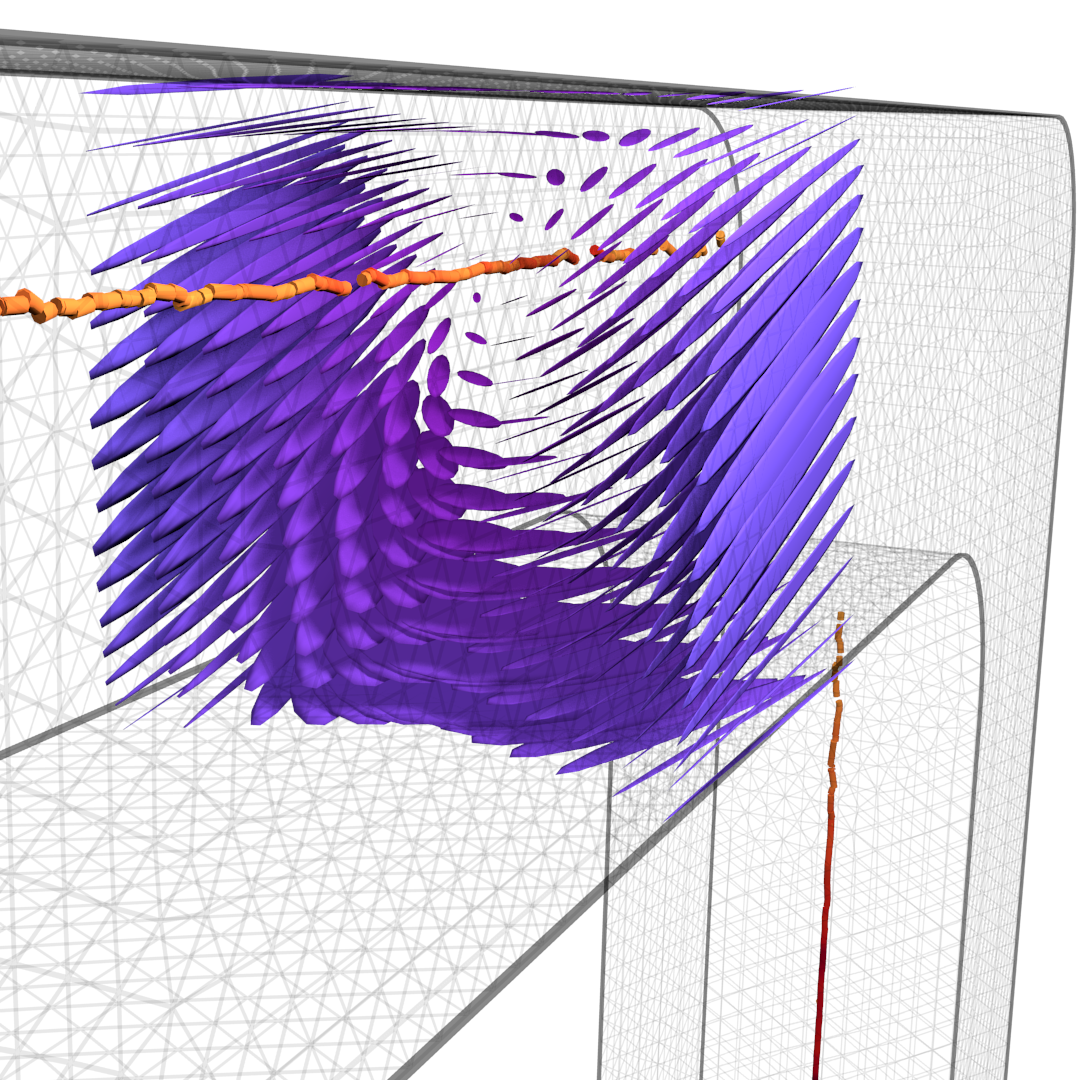
\includegraphics[width=0.22\figurewidth]{figures/hook2_detail2}%
    };

    \node[image, below=of image1, yshift=-0.25cm] (image5)
    {
        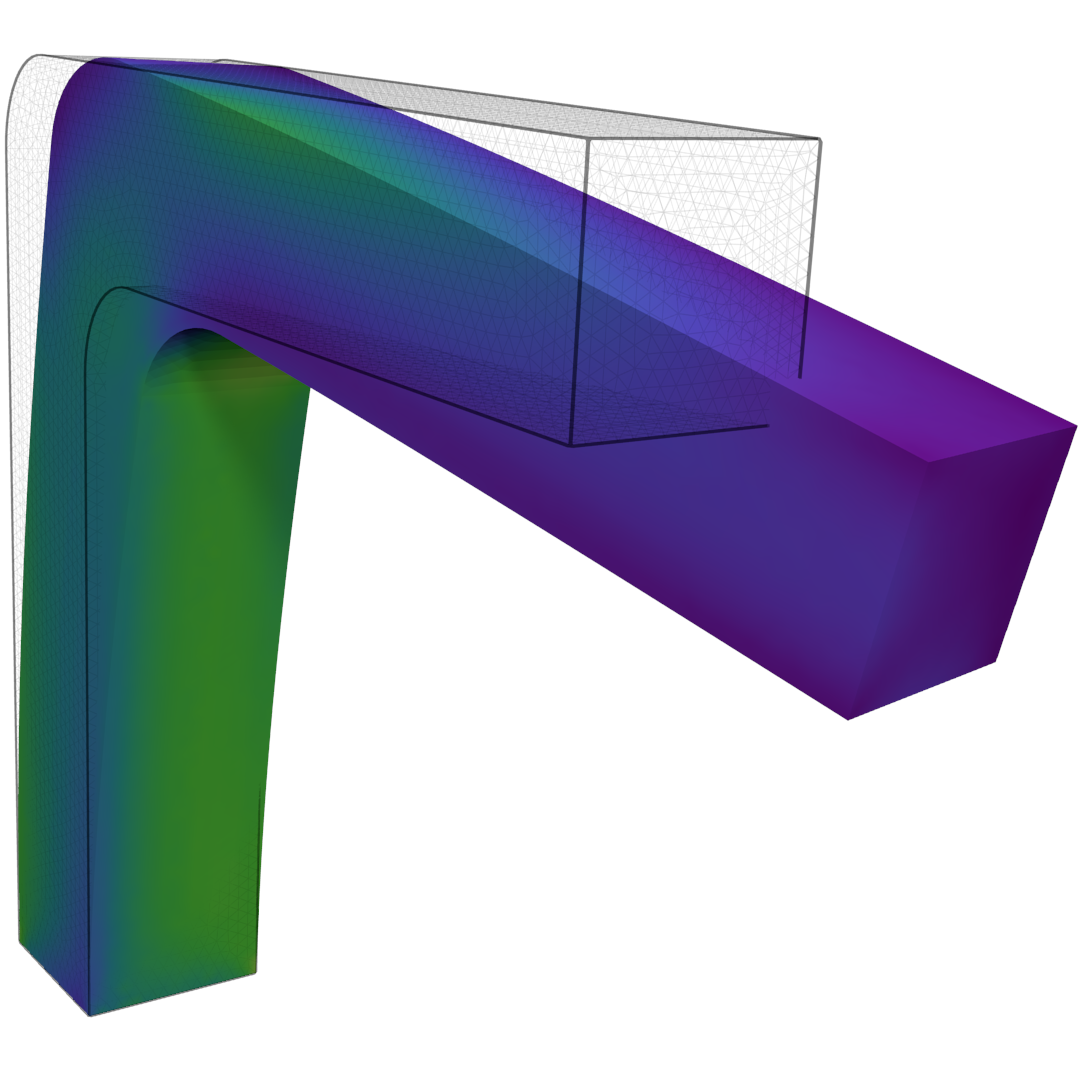
\includegraphics[width=0.22\figurewidth]{figures/hook3_deformation}%
    };

    \node[image, right=of image5, xshift=0.25cm] (image6)
    {
        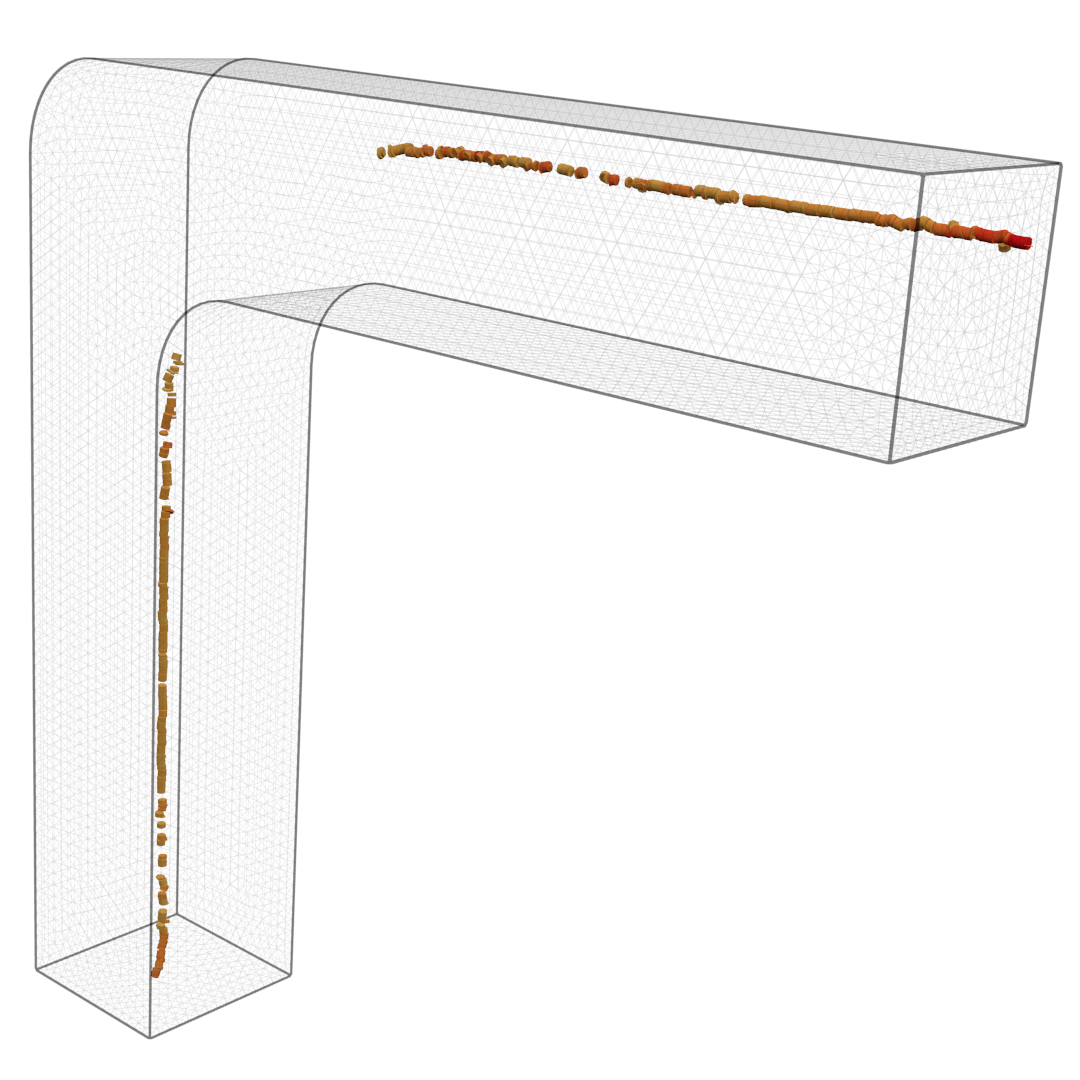
\includegraphics[width=0.22\figurewidth]{figures/hook3_lines}%
    };

    \node[image, right=of image6, xshift=0.25cm] (image7)
    {
        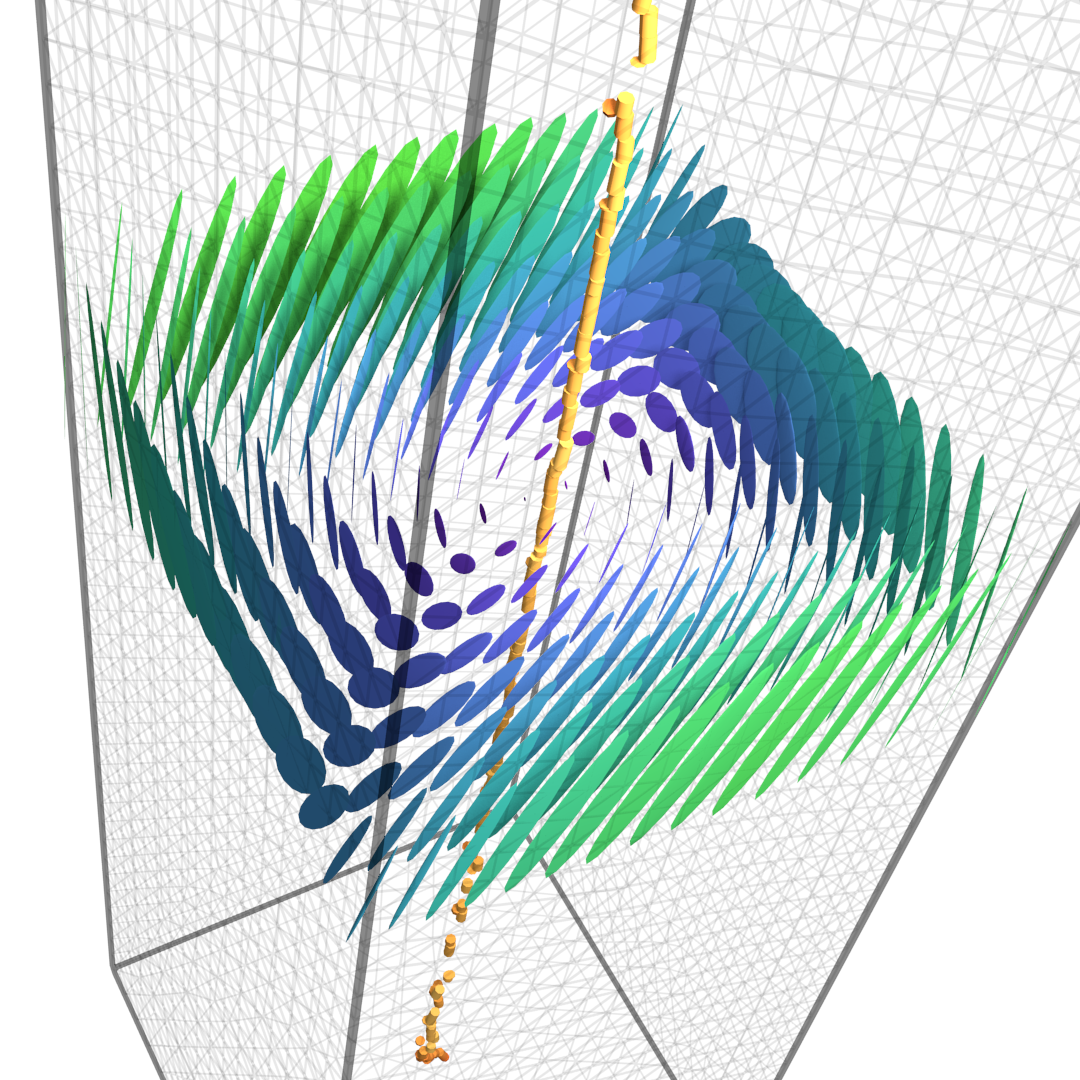
\includegraphics[width=0.22\figurewidth]{figures/hook3_detail1}%
    };

    \node[image, right=of image7, xshift=0.25cm] (image8)
    {
        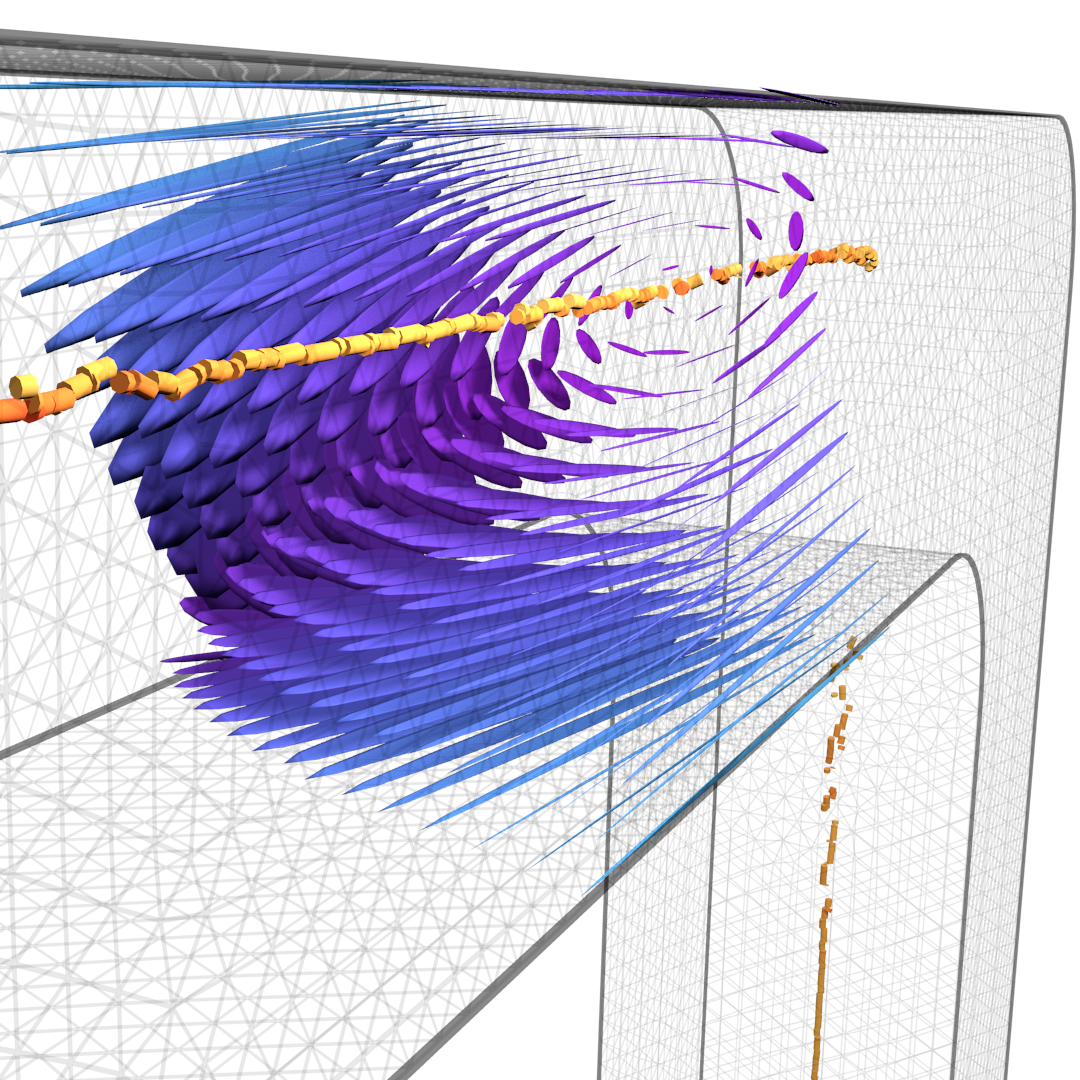
\includegraphics[width=0.22\figurewidth]{figures/hook3_detail2}%
    };

    % This is how you can add a color scale
    \node[anchor=west, xshift=-0.75cm, yshift=-0.1cm] at (image4.east){
        \begin{axis}[
            scale only axis,
            height=3.1cm,
            hide axis,
            domain=1:20,
            colorbar,
            colorbar/width=0.25cm,
            colormap name={cubicyf},
            point meta min=0, point meta max=8e9,
            colorbar style={
                title=$\sigma_{\text{vM}}$,
                scaled ticks=false,
                ytick={0, 8e9}
            }]
        \end{axis}
    };
    \node[anchor=west, xshift=-0.85cm, yshift=-0.1cm] at (image8.east){
        \begin{axis}[
            scale only axis,
            height=3.1cm,
            hide axis,
            domain=1:20,
            colorbar,
            colorbar/width=0.25cm,
            colormap name={rdoryl},
            point meta min=-5, point meta max=11,
            colorbar style={
                title=$\log(s)$,
                scaled ticks=false,
                ytick={-5, 11}
            }]
        \end{axis}
    };

\end{tikzpicture}